\documentclass[10pt,a4paper]{article}

\usepackage[margin=1.05in]{geometry}
\usepackage{setspace,amsmath,amssymb,amsthm}
\usepackage{graphicx,enumitem,titlesec,fancyhdr,microtype}
\usepackage{hyperref}
\graphicspath{{../../drawings/pass2/}{../../drawings/pass1/walk/}}
\hypersetup{colorlinks=true,linkcolor=black,urlcolor=black,citecolor=black}

\titleformat{\section}{\normalsize\bfseries}{}{0em}{}
\titlespacing*{\section}{0pt}{1.35em}{0.5em}

\theoremstyle{plain}
\newtheorem{proposition}{Proposition}
\theoremstyle{definition}
\newtheorem{definition}{Definition}
\theoremstyle{remark}
\newtheorem{observation}{Observation}

\setstretch{1.14}
\pagestyle{fancy}
\fancyhf{}
\fancyhead[L]{\small\itshape Elements of Position}
\fancyhead[R]{\small\itshape III.\ Without a Landing}
\fancyfoot[C]{\small\thepage}
\renewcommand{\headrulewidth}{0pt}

\begin{document}

\begin{center}
\vspace*{1.8em}
{\large Elements of Position}\\[1.4em]
{\LARGE\bfseries III.\ Without a Landing}\\[0.4em]
{\small The residual the operators leave, and what the pair still forces}\\[1.4em]
{\normalsize Justin Erholtz}\\[0.3em]
{\small 12 September 2026}
\end{center}

\vspace{1.0em}

\noindent
\textit{A note.}
Part~II named an entrance residual and then, in places, treated it as dirt on an idealization.
This part writes the residual as an object.
A heading identity is checked against \(u_m\).
A pair identity is checked against \(m\), by Part~I.
Plates L1 and L2 read the recorded tables. They are not a second walk.

\tableofcontents

\section{The leftover of the landing is forced}

Hit \(m\) occurs at step \(j_m=\lceil m\lambda\rceil\) whenever \(m\lambda\) is not an integer,
\(\lambda=\pi/\arctan h\).
The heading has already passed \(m\pi\) by
\[
\varepsilon_m=\arctan(h)\,(1-\{m\lambda\}).
\]

\begin{proposition}
\(u_m=\bigl((-1)^m\cos\varepsilon_m,\;(-1)^m\sin\varepsilon_m\bigr)\).
\end{proposition}

On the recorded kick the first residual is the vertical of the first hit:
\(h_y=-0.00040316\) at \(m=1\).
The continuous-clock detector that waits for \(y>0.05\) and then \(y\le 0\) arrives at the same heading.
The operators do not contain the wall.
A hit is the first sample after the crossing.


\begin{figure}[htbp]
\centering
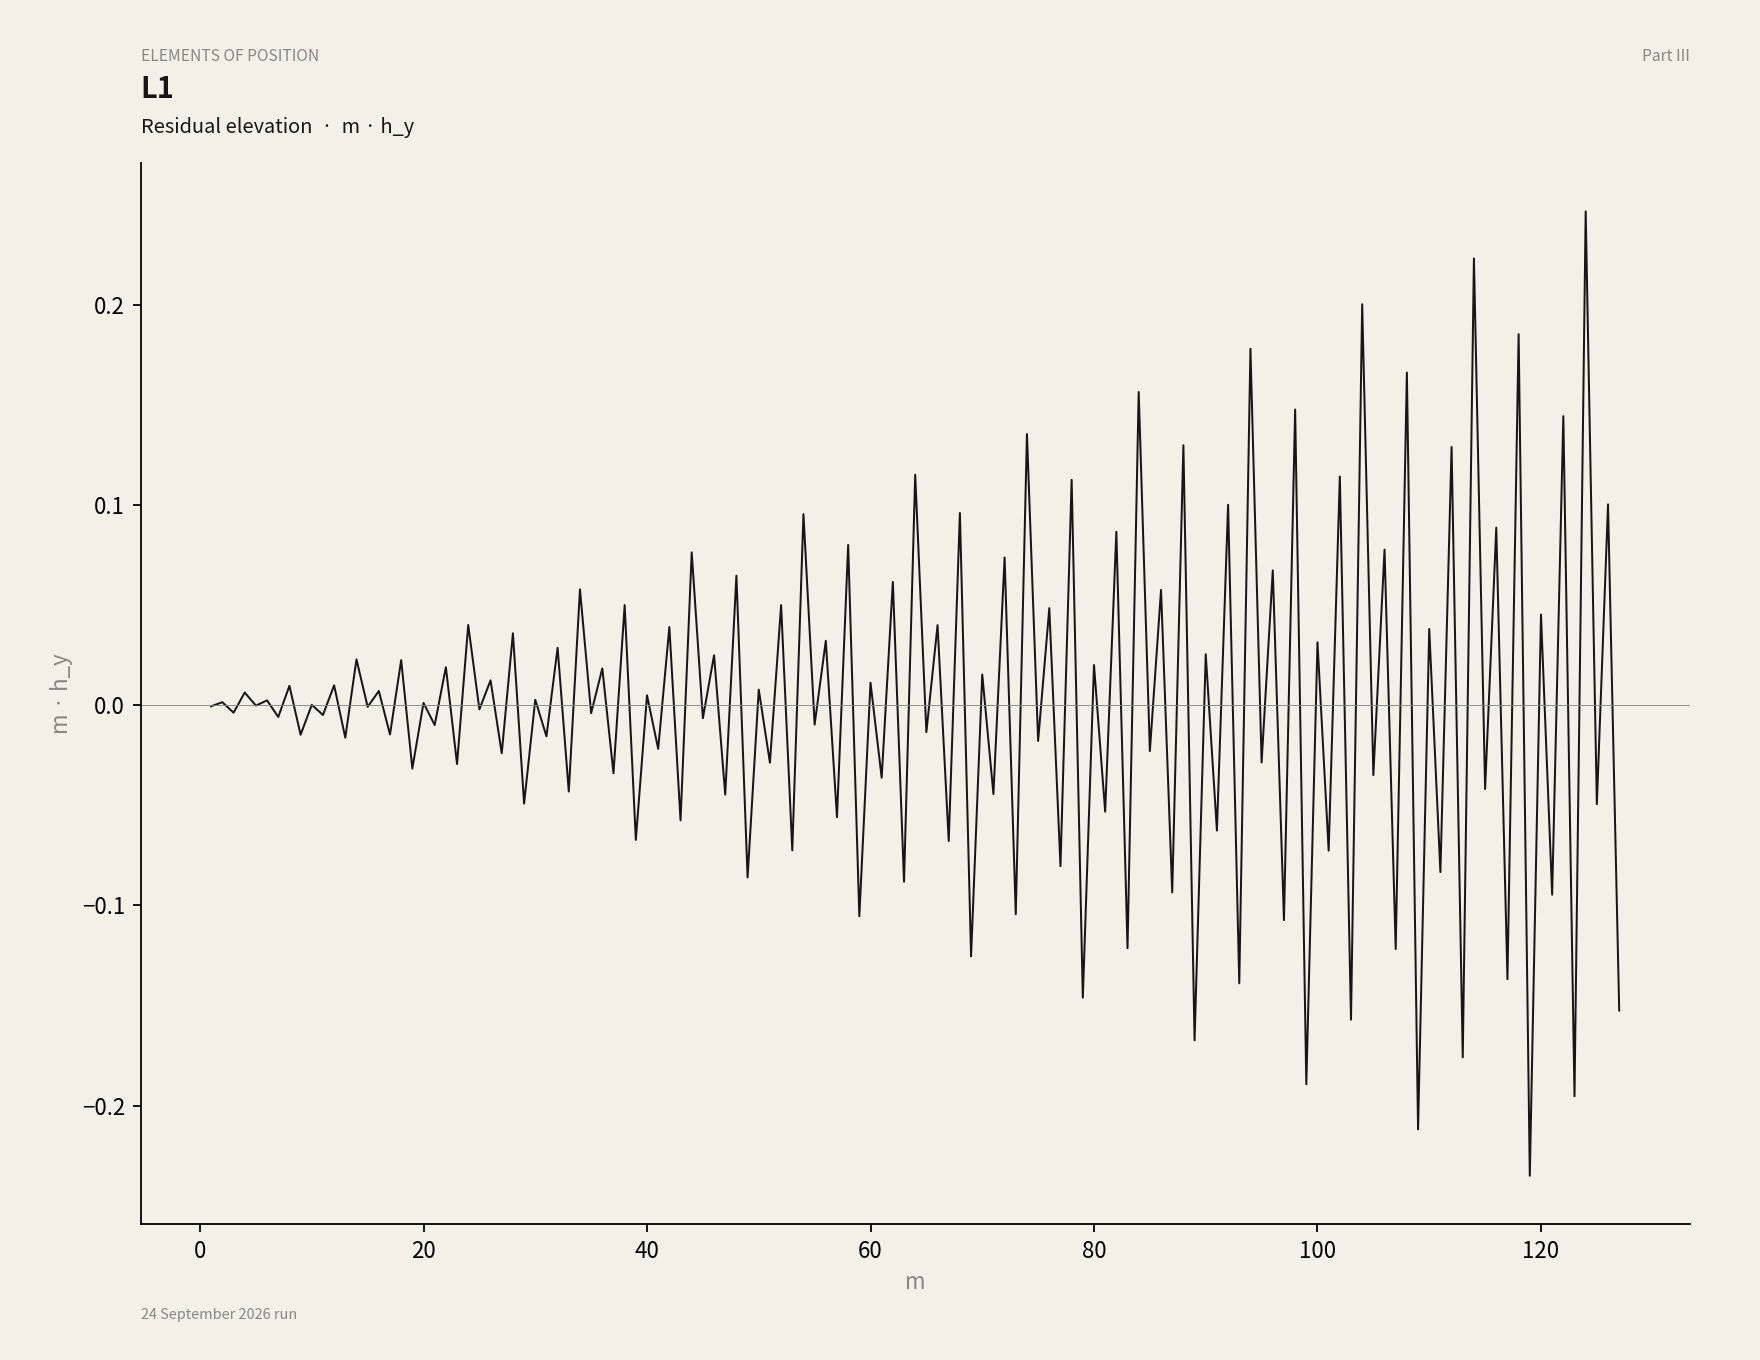
\includegraphics[width=0.92\textwidth]{L1_residual.png}
\caption{Sheet L1. Elevation of $m\cdot h_y$ on the recorded hits. The residual is the object.}
\end{figure}

\begin{proposition}
\(\varepsilon_m=0\) if and only if \(m\lambda\in\mathbb{Z}\).
\end{proposition}

That is the half-turn mix of Part~II, and only that mix.

\section{What does not need a landing}

These are identities of the pair and of inversion.
They use \(u_m\) only as a ray.

\[
|OP_m|\,|OQ_m|=1,\qquad
Q_m=P_m/|P_m|^2,\qquad
\bigl(\tfrac1m,\,m;\,1,\,-1\bigr)=-1,\qquad
\tau(m)=\tfrac{(m-1)^2}{2m}.
\]

The circle on diameter \(OP_m\) meets the unit circle at points whose foot on the ray is exactly \(Q_m\).
Foot error on the recorded headings: \(2\times 10^{-16}\).
The mouth of that kite is \(2\sqrt{1-1/m^2}\).
At the lock the mouth is \(0\).
At the first split it is \(\sqrt{3}\).
It walks toward \(2\) and does not reach \(2\) at any finite hit.


\begin{figure}[htbp]
\centering
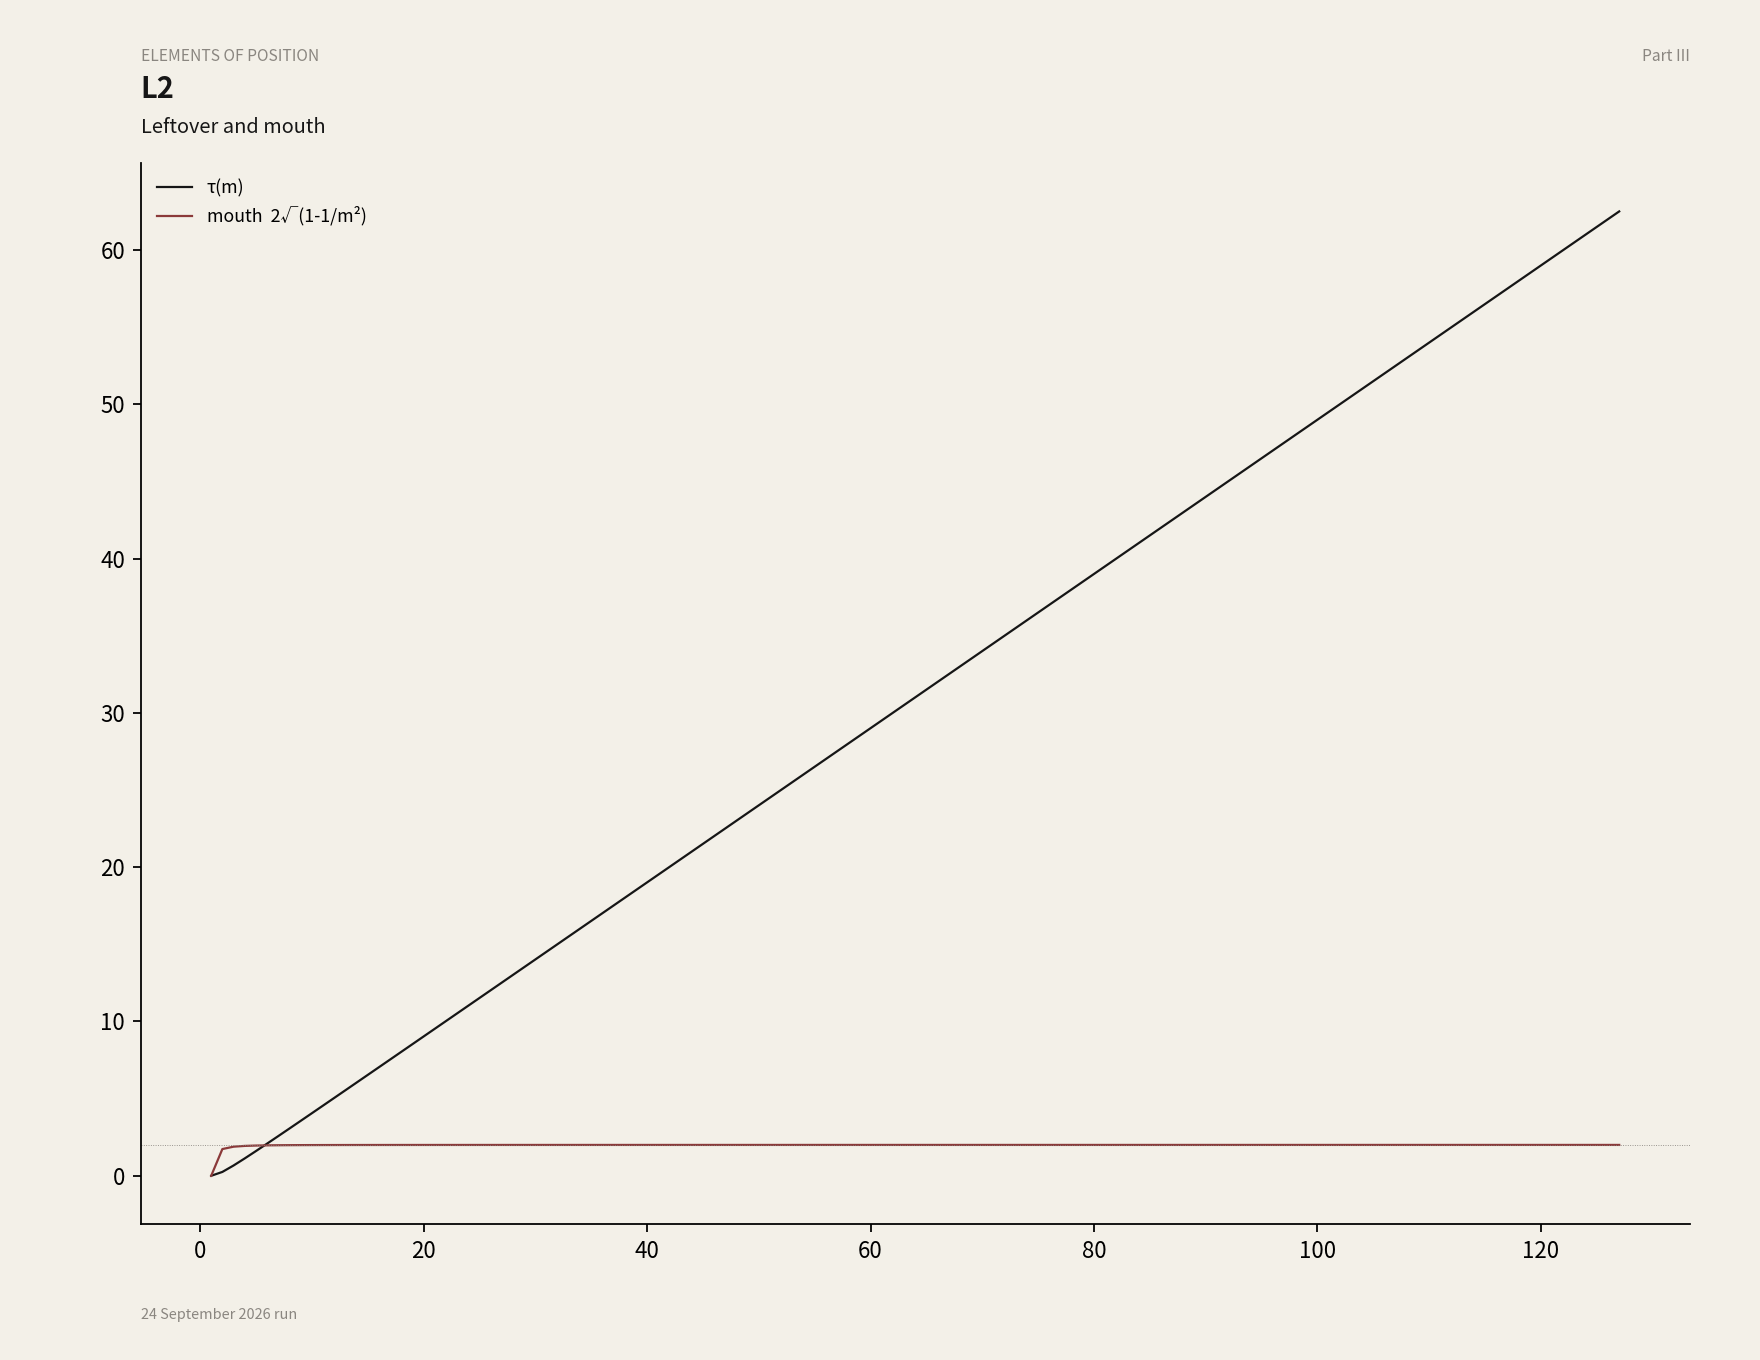
\includegraphics[width=0.92\textwidth]{L2_mouth.png}
\caption{Sheet L2. Leftover climbs. Mouth jumps at the first split and then sits toward $2$.}
\end{figure}

Opposite-wall chords \(|P_m-P_{m-1}|=2m-1\) assume \(u_m=-u_{m-1}\).
The operators deliver \(u_m\cdot u_{m-1}=-\cos(\varepsilon_m-\varepsilon_{m-1})\).
The missing length is of order \(\varepsilon^2\).

\section{The kite factor}

At every hit the pair writes \(1-1/m^2\).
That is the square of half the mouth, and also \(1-|Q_m|^2\).

\[
\prod_{m=2}^{N}\Bigl(1-\frac1{m^2}\Bigr)=\frac{N+1}{2N}.
\]

It walks toward \(1/2\).
Integers only.

Kept only at new inners --- hits whose inner \(1/m\) is not a product of earlier inners --- the same product walks toward a named comparison \(6/\pi^2\).
The name is a sheet reading.
The object is the product of kite factors at those hits.
New inner is primality of the hit index, named as that, not as a narrower ``full web.''

\section{The mix family}

\(T_{a,b}(x,y)=(x-ay,\,y+bx)\), then bind.
Opposite signs return.
Equal \(a=b\) is balance, not a new kind.
Same-sign Euclidean bind does not return.
The minus is the kind.
The residual law rides on whatever kick still returns.

\section{What stands}

Forced at every residual:
the heading formula;
the pair, the inversion, the kite-foot, the right angle at \(X\);
exact closure exactly when \(m\lambda\) is an integer, and only on the half-turn mix.

Forced only as well as two headings agree:
opposite-wall chords, their product, the swap of collinear diameters.

Not granted:
a landing on the cut;
\(\alpha\) of a first block treated as a constant of the operators;
a value of \(4\), or of \(1/2\), or of \(2\), treated as reached at a finite hit.

Where is \(1\)?
It is the lock.
Even there the operators did not land.
They only met themselves.

\end{document}
